%%%%%%%%%%%%%%%%%%%%%%%%%%%%%%%%%%%%%%%%%%%%%%
%                insertmeeting
% 1) Title (something creative & funny?)
% 2) Date (MM/DD/YYYY)
% 3) Location (ex. Hagerty High School)
% 4) People/Committees Present 
% 5) Picture 
% 6) Start Time & Stop Time (ex. 12:30AM to 4:30PM)
%%%%%%%%%%%%%%%%%%%%%%%%%%%%%%%%%%%%%%%%%%%%%%
\insertmeeting 
	{Going Up, Helicopter!} 
	{01/30/22} 
	{Hagerty High School}
	{Annika, Clayton, Falon, James, Jensen, Nathan, Ritam, Samantha}
	{Images/RobotPics/robot.jpg}
	{2:30 - 4:30}
	
\hhscommittee{Multimedia}
\noindent\hfil\rule{\textwidth}{.4pt}\hfil
\subsubsection*{Goals}
\begin{itemize}
    \item Character drawing continues and finding music for the video.

\end{itemize} 

\noindent\hfil\rule{\textwidth}{.4pt}\hfil

\subsubsection*{Accomplishments}
This step of the Promote video requires much more correspondence between members. For each scene, line art would be drawn and the file would be sent to another member who specialized in coloring. Then, through email, the file would be sent back and reviewed. We had to follow this process because Photoshop does not allow multiple people to work on the same file at once. However, this method was efficient in allowing us to complete the frames quickly and save them to the Google Drive to be put into the final editing software: iMovie. We also set aside some time today to look for music to play in the background of our video. We began our search on a website that offers royalty free music, and looked through certain tags to find the right style of music. After some searching, we decided on "Inspire", which is a fitting name for the goal of our PSA. 
 

\begin{figure}[ht]
\centering
\begin{minipage}[b]{.48\textwidth}
  \centering
  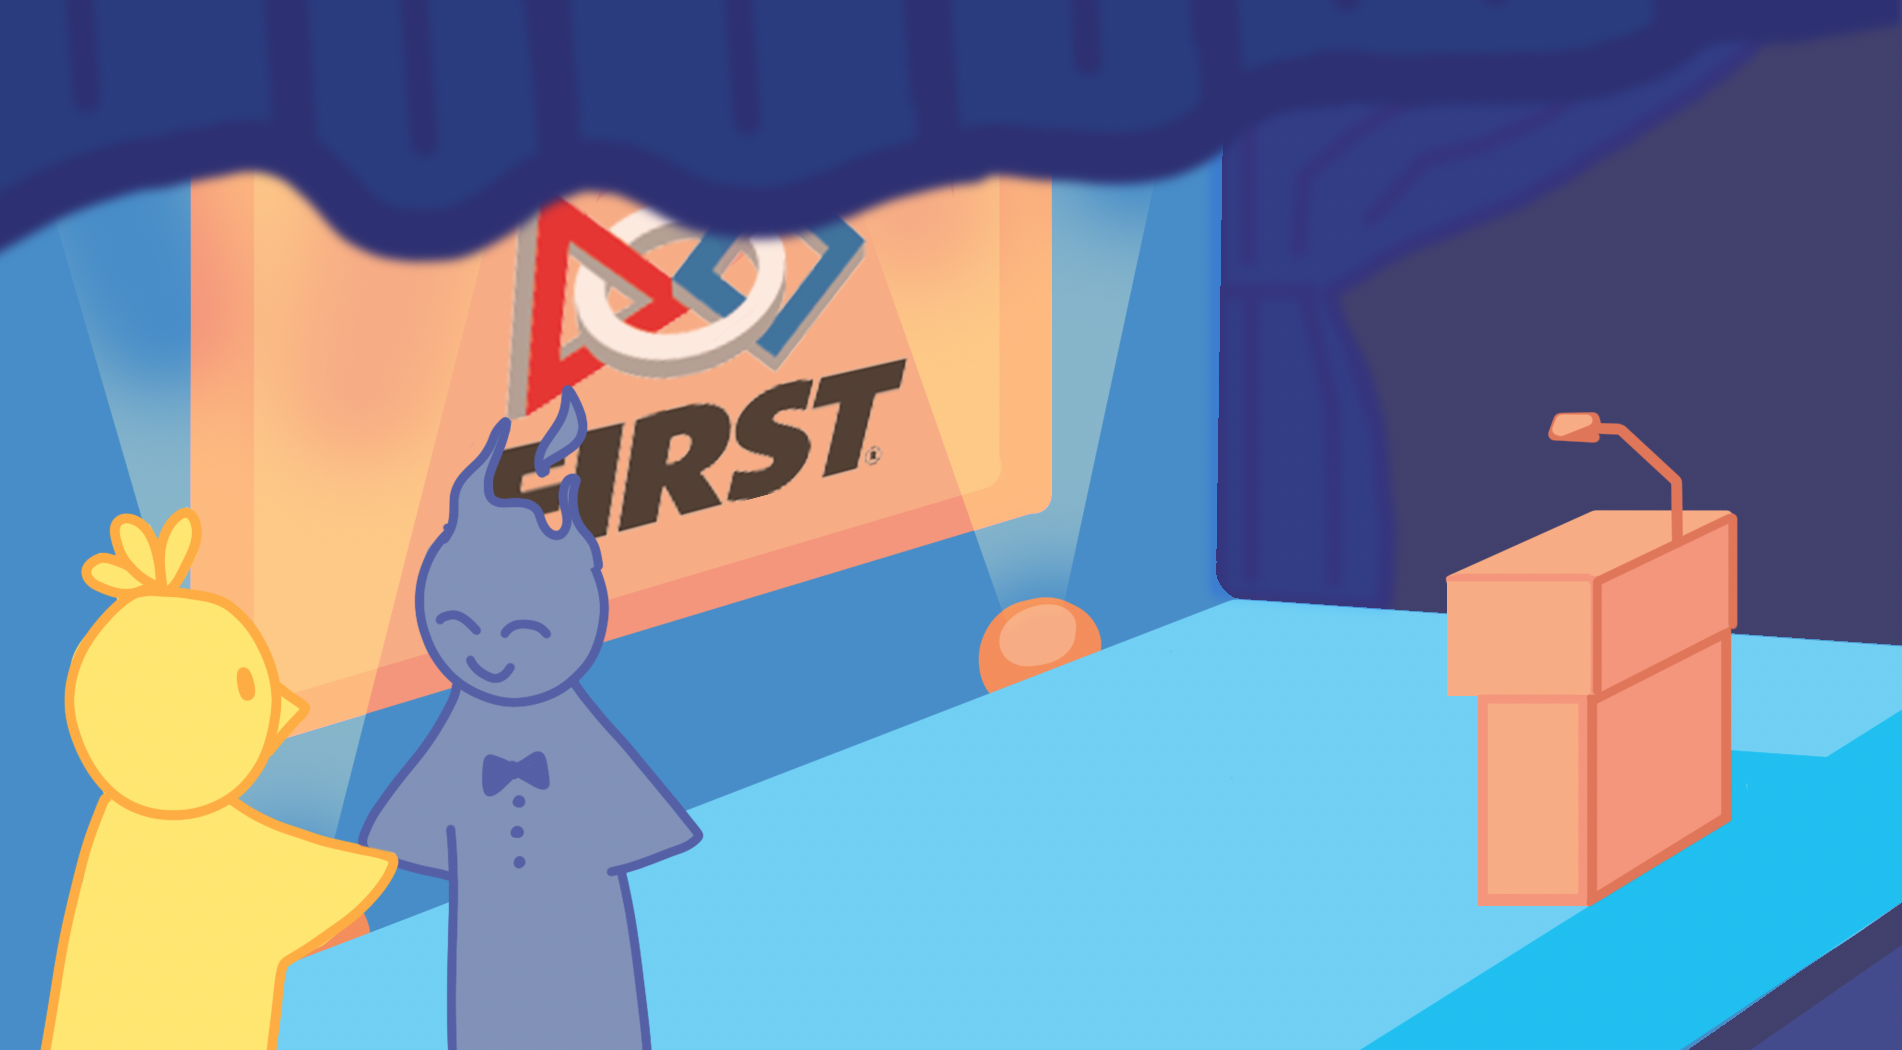
\includegraphics[width=0.95\textwidth]{Meetings/January/01-30-22/1.30.22 - Falon Jones.png}
  \caption{Animating characters}
  \label{fig:013022_1}
\end{minipage}%
\hfill%
\begin{minipage}[b]{.48\textwidth}
  \centering
  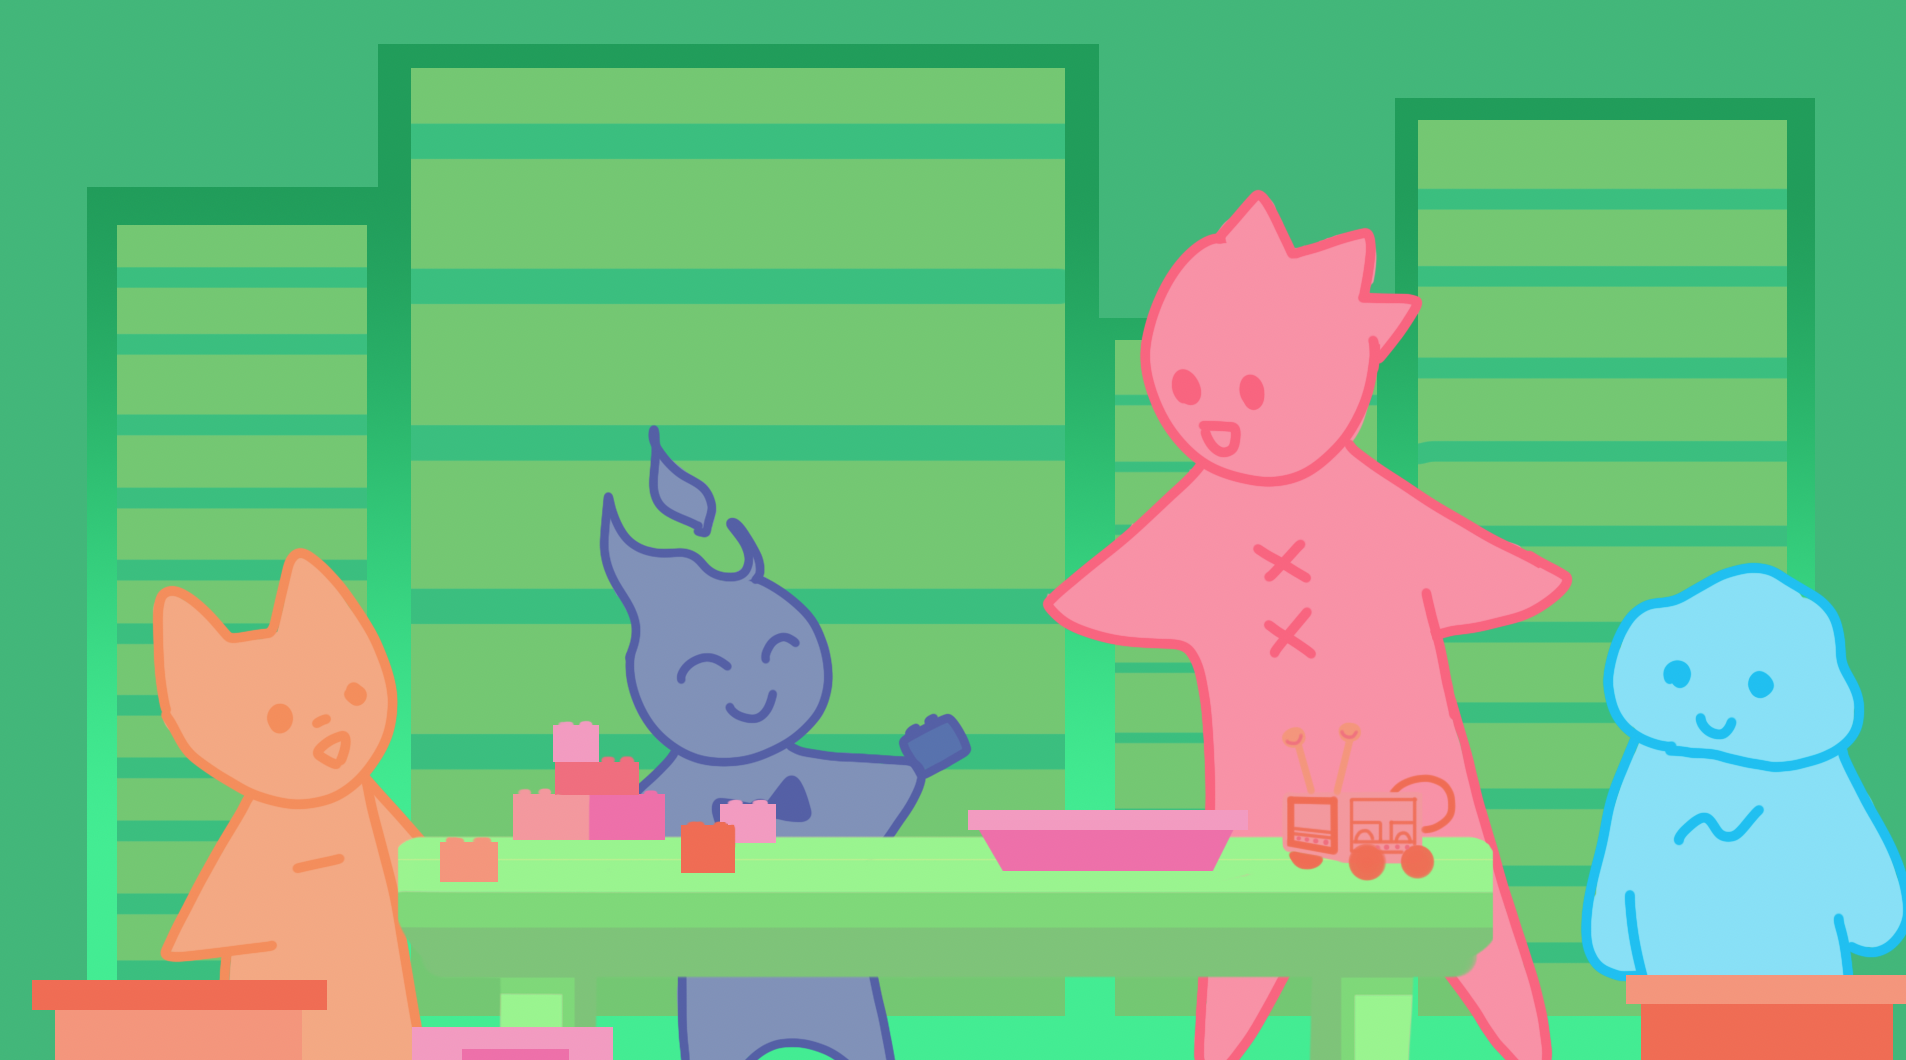
\includegraphics[width=0.95\textwidth]{Meetings/January/01-30-22/1_30_22 - Falon Jones.png}
  \caption{More animation}
  \label{fig:013022_2}
\end{minipage}
\end{figure}

\whatsnext{
\begin{itemize}
    \item Continue to draw characters and record the VoiceOver.
\end{itemize} 
}

